%%%%%%%%%%%%%%%%%%%%%%%%%%%%%%%%%%%%%%%%%%%%%%%%%%%%%%%%%%%%%%%%%%%%%
% PREAMBLE
%%%%%%%%%%%%%%%%%%%%%%%%%%%%%%%%%%%%%%%%%%%%%%%%%%%%%%%%%%%%%%%%%%%%%
%
% The following two commands will generate a PDF that follows all the requirements for submission
% and peer review.  Uncomment these commands to generate this output (and comment out the two lines below.)
%
% DOUBLE SPACE VERSION FOR SUBMISSION TO THE AMS
%\documentclass{ametsocV5}
 \documentclass[twocol]{ametsocV5}

%\journal{jpo}
%\linenumbers
\graphicspath{{../doc/}}
\usepackage[plain]{fancyref}
% \usepackage{xcolor}
\newcommand{\tempS}[1]{}
\newcommand{\twowidth}[0]{4in}
\newcommand{\onewidth}[0]{3.2in}
\newcommand{\mn}[1]{{\sc #1}}
\DeclareGraphicsExtensions{%
    .pdf,.png}
\usepackage{amsmath,amsfonts,amssymb,bm}
\usepackage{mathptmx}%{times}
\usepackage{newtxtext}
\usepackage{newtxmath}


% \bibpunct{(}{)}{;}{a}{}{,}
% \linenumbers
% \newcommand{\myabstract}{}
%
%
%%%%%%%%%%%%%%%%%%%%%%%%%%%%%%%%%%%%%%%%%%%%%%%%%%%%%%%%%%%%%%%%%%%%%
% TITLE
%
% Enter your TITLE here
%%%%%%%%%%%%%%%%%%%%%%%%%%%%%%%%%%%%%%%%%%%%%%%%%%%%%%%%%%%%%%%%%%%%%
\title{Parameterizing non-propagating form drag over rough bathymetry}
%
% Author names, with corresponding author information.
% [Update and move the \thanks{...} block as appropriate.]
%
\authors{Jody M. Klymak \correspondingauthor{Jody Klymak, jklymak@uvic.ca, University of Victoria, Victoria, BC, Canada}}
\affiliation{University of Victoria, Victoria, BC, Canada}

\extraauthor{Dhruv Balwada }
\extraaffil{University of Washington, Seattle, WA, USA}

\extraauthor{Alberto Naveira Garabato}
\extraaffil{University of Southampton, National Oceanography Centre, Southampton, United Kingdom}

\extraauthor{Ryan Abernathey}
\extraaffil{Columbia University, New York, New York, USA}



% \email{jklymak@uvic.ca}

\abstract{}

\begin{document}

\maketitle

%%%%%%%%%%%%%%%%%%%%%%%%%%%%%%%%%%%%%%%%%%%%%%%%%%%%%%%%%%%%%%%%%%%%%
% MAIN BODY OF PAPER
%%%%%%%%%%%%%%%%%%%%%%%%%%%%%%%%%%%%%%%%%%%%%%%%%%%%%%%%%%%%%%%%%%%%%
\section{Introduction}

Goal is to see how we get from isolated bathymetry to rough bathymetry.

\section{Basic runs}

These are just like normal - all rough bottom, dissipation near the bottom. 

\begin{figure*}[htbp]
  \begin{center}
    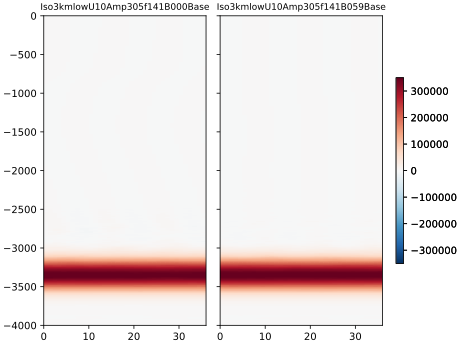
\includegraphics[width=\twowidth]{BaseRunsDiss}
    \caption{Runs with and without beta, Dissipation as function of time (hours) and depth after 10 d of spinup
      \tempS{\footnotesize /Users/jklymak/AbHillInterAnalysis/doc//WorkSummary.ipynb ;
        /Users/jklymak/AbHillInterAnalysis/doc/BaseRunsDiss.pdf.pdf}
      \label{fig:BaseRunsDiss} }
  \end{center}
\end{figure*}


\clearpage

\section{Isolated roughness}



%\begin{appendix}
%%%%%%%%%%%%%%%%%%%%%%%%%%%%%%%%%%%%%%%%%%%%%%%%%%%%%%%%%%%%%%%%%%%%%
% ACKNOWLEDGMENTS
%%%%%%%%%%%%%%%%%%%%%%%%%%%%%%%%%%%%%%%%%%%%%%%%%%%%%%%%%%%%%%%%%%%%%
\acknowledgments

This work was funded under the Office of Naval Research Flow Encountering Abrupt Topography Defence Research Initiative (grant N00014-15-1-2585), and NSERC Discovery Grant 327920-2006.  Thanks to Odessa Murray who manages the High Performance Computing accounts for ONR. ACNG acknowledges the support of the Royal Society and the Wolfson Foundation.  DB acknowledges support from NSF OCE 1756882.


%\subsection{First appendix secondary heading}
%
%\subsection{Second appendix secondary heading}
%
%\subsubsection{First appendix tertiary heading}
%
%\subsubsection{Second appendix tertiary heading}
%
%\paragraph{First appendix quaternary heading}
%
%\paragraph{Second appendix quaternary heading}
%
%\end{appendix}

% Create a bibliography directory and place your .bib file there.
% -REMOVE ALL DIRECTORY PATHS TO REFERENCE FILES BEFORE SUBMITTING TO THE AMS FOR PEER REVIEW



\bibliographystyle{ametsoc2014}
\bibliography{./main.bib}

%%%%%%%%%%%%%%%%%%%%%%%%%%%%%%%%%%%%%%%%%%%%%%%%%%%%%%%%%%%%%%%%%%%%%
% FIGURES-REMOVE ALL DIRECTORY PATHS TO FIGURE FILES BEFORE SUBMITTING TO THE AMS FOR PEER REVIEW
%%%%%%%%%%%%%%%%%%%%%%%%%%%%%%%%%%%%%%%%%%%%%%%%%%%%%%%%%%%%%%%%%%%%%

%
\end{document}
